%% LyX 2.1.2 created this file.  For more info, see http://www.lyx.org/.
%% Do not edit unless you really know what you are doing.
\documentclass[12pt,english]{extarticle}
\usepackage{amsmath}
\usepackage{fontspec}
\setmainfont[Ligatures=TeX]{Times New Roman}
\usepackage[a4paper]{geometry}
\geometry{verbose,tmargin=2.5cm,bmargin=2.5cm,lmargin=4cm,rmargin=2.5cm}
\setlength{\parskip}{\bigskipamount}
\setlength{\parindent}{0pt}
\usepackage{color}
\usepackage{babel}
\usepackage{float}
\usepackage{booktabs}
\usepackage{pdfpages}
\usepackage{graphicx}
\usepackage{setspace}
\usepackage[authoryear]{natbib}
\usepackage{nomencl}
% the following is useful when we have the old nomencl.sty package
\providecommand{\printnomenclature}{\printglossary}
\providecommand{\makenomenclature}{\makeglossary}
\makenomenclature
\setstretch{1.5}
\usepackage[unicode=true,pdfusetitle,
 bookmarks=true,bookmarksnumbered=false,bookmarksopen=false,
 breaklinks=false,pdfborder={0 0 0},backref=false,colorlinks=false,pdfpagemode=FullScreen]
 {hyperref}

\makeatletter

%%%%%%%%%%%%%%%%%%%%%%%%%%%%%% LyX specific LaTeX commands.
%% Because html converters don't know tabularnewline
\providecommand{\tabularnewline}{\\}
%% A simple dot to overcome graphicx limitations
\newcommand{\lyxdot}{.}


%%%%%%%%%%%%%%%%%%%%%%%%%%%%%% Textclass specific LaTeX commands.
\usepackage{enumitem}		% customizable list environments
\newlength{\lyxlabelwidth}      % auxiliary length 
\newenvironment{lyxcode}
{\par\begin{list}{}{
\setlength{\rightmargin}{\leftmargin}
\setlength{\listparindent}{0pt}% needed for AMS classes
\raggedright
\setlength{\itemsep}{0pt}
\setlength{\parsep}{0pt}
\normalfont\ttfamily}%
 \item[]}
{\end{list}}

%%%%%%%%%%%%%%%%%%%%%%%%%%%%%% User specified LaTeX commands.
\usepackage{pdflscape}
\usepackage{abstract}
\usepackage{setspace}
\usepackage[nottoc]{tocbibind}
\pagenumbering{roman}
\providecommand{\BIBand}{and}

\makeatother

\begin{document}
\noindent \begin{center}
{\LARGE{}\vphantom{}\vphantom{}\vphantom{}\vphantom{}Influence
of Geographic Isolation on the Resistance of Norway spruce (}\emph{\LARGE{}Picea
abies}{\LARGE{}) to }\emph{\LARGE{}Heterobasidion parviporum}{\LARGE{}}\\
{\LARGE{}\vfill{}
}
\par\end{center}{\LARGE \par}

\noindent {\small{}........................Thesis submitted for a
M.Sc. degree in Forest Sciences and Business}{\small \par}

\noindent \begin{flushleft}
{\small{}\hspace{65bp}University of Helsinki }\\
{\small{}\hspace{65bp}Dept. of Forest Sciences }\\
{\small{}\hspace{65bp}May, 2015 }\\
{\small{}\hspace{65bp}}\\
{\small{}\hspace{65bp}Erik Stewart}
\par\end{flushleft}{\small \par}

\thispagestyle{empty}\renewcommand{\abstractname}{}\renewcommand{\absnamepos}{empty}
\begin{quotation}
\noindent \pagebreak{}

\includepdf{C:/Users/user/Documents/Courses/Thesis/Thesis_abstract_page_Stewart}\end{quotation}
\begin{abstract}
\pagebreak{}

\pagenumbering{roman} \setcounter{page}{1}

\singlespacing

\noindent \tableofcontents{}

\noindent \printnomenclature{}

\pagebreak{}\end{abstract}
\begin{lyxcode}
\pagenumbering{arabic} \setcounter{page}{1}
\end{lyxcode}

\section{Introduction }

Norway spruce (\emph{Picea abies}) is a commercially significant
conifer with a ubiquitous distribution throughout most of Finland.
In Finland, Norway spruce accounts for 30\% of total forest growing
stock volume \citep{EsaYlitalo2013}. Because of its significant impact
on the Finnish economy, it is important to understand and to address
issues which negatively affect the growth and production of Norway
spruce.

The most devastating pathogen affecting the growth of Norway spruce
in the northern hemisphere is butt rot caused by the \emph{Heterobasidion annosum}
\emph{sensu lato. (s.l.)} species complex. Damages to forest production
in Europe from \emph{H. annosum s.l.} is greater than 800 million
euros annually; as such, it is important to study the pathogen and
host to better understand the complex nature of infection biology
and resistance factors, which hold the potential for mitigating losses
and improving forest yields in areas where \emph{H. annosum s.l.}
is prevalent \citep{Stenlid1998}


\subsection{Norway spruce (\emph{P. abies}) in Northern Europe}

Norway spruce, despite its name, established itself in northern Europe
via eastern Finland approximately 6,500 years ago \citep{Seppa2009}.
However, in this relatively short period of time, Norway spruce has
become one of the most dominant forest trees in of northern Europe,
owing partially to the fact that Norway spruce has high genetic plasticity
\citep{Chen2012,Reich1996}. Although most populations of \emph{P.
abies }in northern Europe have been established relatively recently
considering the species emerged millions of years ago, some populations
in ice free areas of western Scandinavia likely survived the last
ice age approximately 18,500 years ago \citep{Tollefsrud2008}.



Norway spruce is a shade tolerant conifer, which grows at the final
stages of ecological succession. A tolerance for shade allows \emph{P.
abies }to establish in mixed forests in the understory during early
stages of growth, with increased growth opportunistically to fill
in canopy gaps as they occur \citep{Jonsson1990}. Initial growth
of the tree is slow, but increases between 20-60 years of age \citep{Kostler1956}.
Generally, \emph{P. abies }lives for 200 years in the southern areas
of its range, but can survive up to 400 years in the northern areas
of its range \citep{Kostler1956}. The root systems of Norway spruce
are superficial, making the tree susceptible to windfall \citep{Kostler1956}.
In Finland, Norway spruce is found throughout most of the country.
Only small areas in the very northern parts of Finland in the Arctic
Circle are devoid of \emph{P. abies. }Unsurprisingly, the near ubiquitous
presence of \emph{P. abies} throughout Finland and Scandinavia has
led to it becoming one of the most important commercial forestry crops
in northern Europe. 


\subsection{Biology and Epidemiology of \emph{H. annosum s.l.}}

The \emph{H. annosum s.l. }species complex is comprised of several
inter-sterile groups of species, each with differing host preferences.
In Europe, three distinct mating types are recognized: \emph{Heterobasidion
annosum sensu stricto}, \emph{Heterobasidion parviporum}, and \emph{Heterobasidion
abietinum, }with host preference for pines (\emph{Pinus} \emph{spp.}),
spruce (\emph{Picea spp.}), and firs (\emph{Abies spp}.), respectively
\citep{Korhonen1998}. In North America, two \emph{H. annosum s.l.}
intersterility group are recognized; \emph{Heterobasidion occidentale,
}and \emph{Heterobasidion irregulare}. 

\emph{H. annosum s.l}. has the ability to infect a broad range of
coniferous trees, as well as some angiosperms. \emph{H. annosum s.l.}
are selective necrotrophs, which causes damage by degrading lignin
and cellulose in host trees; no cures are available after infection
has been established within a host, and death of the host tree will
occur eventually due either to the pathogen or other environmental
factors, such as wind throw in hosts which have compromised structural
integrity due to the effects of the infection. \emph{H. annosum s.l.
}are also effective saprotrophs.\emph{ }However, the degradation
of host tissues to the point of lethality may take several decades.
Due to the mortal nature of infections by \emph{H. annosum s.l., }knowledge
of the life-cycle and infection biology of the pathogen is critical
to understanding how best to deal with the pathogen in areas where
\emph{H. annosum s.l. }present a problem in forestry industries. 

Despite a preference for specific hosts, several species within the
\emph{H. annosum s.l.} complex are able to infect other than their
preferred hosts, albeit with less efficiency \citep{Garbelotto2013}.
The different species of the \emph{H. annosum s.l. }complex\emph{
}are generally unable to hybridize with other species within the \emph{H.
annosum s.l }species complex, with genetic control over inter sterility
regulated by at least five genes \citep{Garbelotto2013,Chase1990}.
However, limited hybridization has been observed, mostly in laboratory
settings between the North American isolates \citep{Garbelotto1993}.
A study by \citet{Garbelotto2007} speculated that little to no observations
of hybrids in natural settings is primarily due to ecological constraints,
and higher competition from pure strains within the species complex. 


\subsubsection{Distribution of \emph{H. annosum s.l.} in Europe}

\emph{H.} \emph{annosum s.l. }is widespread throughout most of the
northern hemisphere. In Europe, the three intersterile groups of \emph{H.
annosum s.l. }dominate in areas where their respective host trees
are found. The European P-type intersterility group (\emph{H. annosum
s.s.}) is found throughout most of Europe, with upper limits to its
extent in the southern to central areas of Finland, despite the presence
of suitable hosts throughout the further northern areas of Europe
\citep{Korhonen1998a}. The S-type intersterility group (\emph{H.
parviporum) }is found further north in Europe than that of the P-type,
but its southern extent generally restricted by lack of suitable hosts
in the most of the more southern parts of Europe \citep{Korhonen1998a}.
The northernmost observations of \emph{H. parviporum} have occurred
just south of the northernmost distribution of \emph{P. abies} in
Finland, at approximately 68º N. Although the S-type intersterility
group has been noted in these northernmost regions, it is not considered
to be a problem in mechanized forestry situations, and incidences
of infections are rare. In contrast with the other two intersterility
groups, the F-type intersterility species of the pathogen (\emph{H.
abitenium) }is only found in southern and central Europe, with upper
limits to its distribution restricted by suitable its host species
range \citep{Korhonen1998a}. However, understanding of the ecological
constraints including temperature regimes which limit the distribution
of these pathogens from areas where suitable hosts are found, such
as in far northern Europe, is lacking \citep{Witzell2011,Korhonen1998a}. 


\subsubsection{Spread and Infection of \emph{H. annosum s.l.}}

\emph{H. annosum s.l. }cannot generally infect healthy, undamaged
tree tissues. In areas where conifers are intensively harvested and
managed, mechanical damages due to forestry related activities provide
new surfaces for inoculations, and exacerbate the problem of \emph{H.
annosum s.l.}, leading to high rates of infection and heavy losses.
The primary way in which new infections are established in areas where
commercial harvesting of forest trees is done is via basidiospore
deposition onto freshly cut stump surfaces \citep{Redfern1998}. The
actual infection process begins when a spore or mycelia reach a suitable
host substrate. Adhesion of spores requires suitable substrate, generally
in the form of a fresh wound exposing living tissues in host tree,
or a stump through which subsequent spread to adjacent trees can occur.
Germination of spores occurs when spores land onto suitable host tissues,
and environmental conditions are sufficient for the survival of the
spores \citep{Redfern1998,Redfern1993}. After infection has been
established, \emph{H. annosum} \emph{s.l. }utilizes lignin and cellulose
as primary carbon sources for growth and proliferation within host
tissues. However, \emph{H. annosum s.l. }can also utilize other sources
of carbon as well \citep{Korhonen1998}.

Other methods by which \emph{H. annosum s.l. }spreads is via mycelial
growth within suitable host substrate, or in very limited distances
throughout soils. Infections can occur in the immature roots of host
trees, as this is the natural vector by which the pathogen spreads
\citep{Asiegbu1995,Johansson1985a}. \emph{H. annosum s.l. }does not
have the ability to grow far in soil without suitable host substrate.
However, root systems of an infected tree which are near to neighboring
tree's root systems, or which are grafted with the roots of another
tree can pass mycelium from the infected tree to the root systems
of another tree. Contact between roots of neighboring trees is also
an important natural vector for the transmission of \emph{H. annosum
s.l. }to uninfected trees within the same stand, and to subsequent
generations in instances where stumps and remaining root tissues from
infected trees are left in place \citep{Garbelotto2013,Asiegbu2005,Woodward1998}. 

Reproduction of \emph{H. annosum s.l. }requires that two homokaryotic
strains of differing genetic origin and with compatible mating loci
fuse to form a heterokaryotic mycelium containing the genetics of
both parent strains. With sufficient climate and access to nutrients,
the heterokaryotic mycelium can form a basidiocarp, generally on the
lower portion of infected trees, although fruiting has been induced
in laboratory settings as well \citep{Woodward1998}. In addition
to infection from sexually produced basidiospores, conidiospores,
an asexual spore produced by \emph{H. annosum s.l. }can also start
new infections, but are not the primary source of new infections. 


\subsubsection{Control of \emph{H. annosum s.l.}}

Various biotic and abiotic methods of control are used to attempt
to reduce the prevalence and damage done to trees by \emph{H. annosum
s.l. }In modern, highly mechanized forest product production, one
of the key routes for new infections of Heterobasidion is a byproduct
of the harvest and maintenance of trees; mechanically created wounds
on trees provides access to suitable host tissues for basidiospores,
although most new infections occur on stumps leftover from logging
operations\citep{Makinen2007,Thor2005,Woodward1998}. Primary methods
for control of \emph{H. annosum s.l. }include the careful use of equipment
and attempts to minimize damage due to anthropogenic factors. Post-harvest
stumps left in place provide an ideal suitable host substrate for
\emph{H. annosum s.l. }Thus, the most efficient and widely utilized
control methods address the issue of suitable host tissue on freshly
cut stumps by means of chemical, biotic, or abiotic control in areas
where infections have not been previously noted. However it is very
difficult to control spread of \emph{H. annosum s.l. }in areas where
the pathogen has previously been established; in areas where prior
generations were infected, stumping after the harvest of the current
generation may be insufficient for controlling spread of \emph{H.
annosum s.l. }to the subsequent generations \citep{Piri2003,Piri1996}.
Chemical control includes treatment of freshly cut stumps with urea,
borax, or a fungicidal product like propiconizole, which can all
be effective at reducing the likelihood of subsequent infection from
\emph{H. annosum s.l. }spores \citep{Garbelotto2013,Nicolotti1999,Woodward1998}.
A typical biotic treatments for the control of \emph{H. annosum s.l.
}includes the application of saprotrophic fungi \emph{Phlebiopsis
gigantea, }which colonizes available substrate (generally stumps)
and out competes \emph{Heterobasidion spp}. \citep{Garbelotto2013,Nicolotti1999,Woodward1998}.
Silvicultural practices which are used to reduce the damage from \emph{H.
annosum s.l. }includes removal of stumps and associated root tissues,
which provide an unchallenged substrate for infections to occur on
for a period of time after harvest when stump surfaces are susceptible
\citep{Vasaitis2008}. Harvest of stumps and removal of sources of
host material suitable for inoculation has proved to be effective
in reducing the subsequent infections and rot \citep{Oliva2010}.


\subsection{Defense Systems and Resistance in Conifers }

Conifers have a variety of defense systems for dealing with both biotic
and abiotic threats. The major defense systems which conifers possess
for dealing with pathogens are constitutive and inducible defenses.
Structural, or constitutive defenses include tissues, structures,
and chemicals present in parts of the tree which either prevent or
reduce the possibility or severity of infection by a pathogen. Induced
defenses are initiated locally and/or systemically upon the recognition
of a pathogen, and include a variety of possible defense actions including
secondary metabolite production, priming of system wide defenses,
and changes to physical structures of the tree. Genetic defenses represent
gene level interactions between plant and pathogen, and can confer
increased resistance to a pathogen or outright immunity, depending
on the tree and pathogen. The constitutive and induced systems of
defense present in conifers are not mutually exclusive of one another,
and interact with components of the other systems of defense within
the tree on some level. 


\subsubsection{Constitutive Defenses in Conifers }

Constitutive defenses present throughout conifers include various
types of tissues and structures which are produced during regular,
unchallenged growth. Bark represents the outermost layer of defense
in a conifer, and is comprised of several distinct tissues: periderm,
cortex, phloem and cambial tissues. The periderm is highly suberized
and hydrophobic, which helps to inhibit adhesion and germination of
fungal spores \citep{Pearce1996}. In most cases, it is not possible
for a fungal pathogen to actively infiltrate intact outer bark tissues,
a notable exception being some species of fungi in the family \emph{Armillaria
}which can penetrate outer defenses \citep{Pearce1996}. However,
not all structures within the bark can adequately resist fungal invasion;
in a study conducted by \citet{Lindberg1991},\emph{ H. parviporum
}was able to establish infections reaching the xylem in all test subjects
with the rhytidome and phellem removed, with inner bark tissues still
intact. 

Features present in the phloem tissues which allow the \emph{P. abies}
to resist damages and pathogen includes polyphenolic parenchyma cells,
and lignified cells. Polyphenolic parenchyma (PP) cells are present
throughout the trees phloem tissues, and store phenolic compounds
which are released if the cells are damaged by wounding either from
mechanical forces or via pathogen growth. Phenolic compounds have
various anti-microbial properties, and resistant clones of \emph{P.
abies} have been shown to have higher amounts of PP cells than susceptible
clones \citep{Franceschi1998}. Xylem tissues include some similar
defense mechanisms to cells in phloem tissues. Lignified cells within
the xylem increase the mechanical strength of a tree, and are more
resistant to fungal infections. However, much higher portions of parenchyma
cells exist within the xylem in conifers, predominantly in the form
of xylem rays. PP cells are also present in large numbers in the xylem
tissues. Further barriers to damage from pathogens or mechanical forces
include large amounts of lignified and suberized tissues.

Sapwood tissues have a variety of constituent and structural defenses,
as well as the ability to induce defenses in response to a pathogen.
For example, the sapwood tissues in Norway spruce which are more resistant
to fungal infection have larger polyphenolic parenchyma cells, which
can contribute to differences in resistance levels of the phloem in
individual trees depending on the resistance of a given phenotype
\citep{Nagy2004}. Trees also create barriers in response to pathogens,
compartmentalizing both axially and radially in response to damages
or detection of a pathogen. Increases to lignification near affected
tissues, plugging of vascular tissues, and programmed cell death are
utilized by the tree to attempt to exclude the pathogen from vulnerable
areas within the host. 


\subsubsection{Inducible Defenses in Conifers}

In addition to the compartmentalization of tissues surrounding a wound
or pathogen within the sapwood, a reaction zone surrounding initial
wound is also created, which is characterized by increased levels
of lignin in surrounding tissues, increased production of phytoalexins,
free radical production from oxidative bursts, and increases in other
chemicals which have antimicrobial properties \citep{Kovalchuk2013,Pearce1996}
Increases in accumulation of antimicrobial compounds in the reaction
area help to restrict further progression of pathogens or damages
which caused the response and compartmentalization of the area in
the first place. The hypersensitive response is the activation of
programmed cellular death in localized areas in response to a pathogen;
however, in the epidemiology of pathogens with necrotrophic lifestyles,
such as \emph{H. annosum s.l.}, the hypersensitive response is ineffective
at stopping an infection. 

\begin{spacing}{1.5}
\noindent Non-specific chemical based defenses in conifer periderm
and sapwood tissues include oleoresin based defenses, increased lignification,
as well as accumulation of antimicrobial chemicals which are produced
during normal plant growth, referred to as phytoanticipins \citep{VanEtten1994}.
Oleoresins are present in sapwood tissues during the normal growth
of many conifer species, and are produced by a variety of specialized
cells depending on the genus. For example \emph{Pinus spp. }have well
developed resin duct tissues, whereas \emph{Abies spp. }produce resin
blisters; \emph{Picea spp.} lack centralized traumatic resin ducts,
and show low levels of constituent monoterperne cyclase activity \citep{Lewinsohn1991}.
However, oleoresin production can greatly increase in response to
wounding or pathogenic attack in genus such as \emph{Picea }\citep{Lewinsohn1991}.
Because oleoresins are produced both in normal growth as well as in
response to abiotic or biotic stresses, it is appropriate to consider
oleoresins as an induced defense strategy as well as a constitutive
one. Phytoalexins are molecular compounds produced in response to
a pathogen, and include a broad range of low molecular weight compounds;
however, true phytoalexins are not known in conifers, but increased
accumulation of phytoanticipins and antimicrobial compounds in response
to pathogens has been observed in conifers \citep{Bonello2006}. Lignans,
stilbenes and terpenoids are phytoalexin-like compounds produced in
\emph{P. abies} and other \emph{Picea spp}. in response to fungal
challenge \citet{Pearce1996}. 
\end{spacing}

Upon infection with \emph{H. annosum s.l.}, broad changes occur in
both the host and pathogen. Specific elicitors detected by a susceptible
host can initiate changes to the physiology of the host both locally
and systemically. Changes in the host include increased production
of secondary metabolites in response to the pathogen. Similarly, once
the pathogen begins to encounter resistance, it can produce compounds
which assist in overcoming the host defense systems. A study by \citet{Swedjemark2007}
found that the priming of resistance by prior inoculation of \emph{H.
parviporum }in Norway spruce had significant effects on reducing the
subsequent necrosis and fungal growth in subsequent inoculations.
Other factors can prime host tree defenses, prompting physiological
changes which confer enhanced resistance to pathogens. Herbivory,
volatile organic compounds, and colonization of the host with certain
types of rhizobacteria or mychorrizal fungi also have the potential
to prime defenses in conifers \citep{Eyles2010}. 

In addition to low molecular weight compounds produced for defenses,
conifers also utilize protein based defenses in response to pathogens.
These protein defenses are known as pathogenesis-related proteins
(PR-proteins), and include proteins across seventeen well defined
families (PR1-PR17), as well as several other classes of less well
understood hypothesized PR-proteins families (PR-18, PR-19) \citep{Kovalchuk2013,Veluthakkal2010}. 

A variety of signaling molecules are important in the induced defense
in conifers. Methyl-jasmonate is an important signaling molecule (produced
when a tree is under attack) which induces a wide variety of changes
to conifer tissues, including traumatic resin duct formation, and
increased production of terpenoid based resin defenses\citep{Martin2002,Hudgins2004,Hudgins2004a,Hudgins2003}.
Salicylic acid is important for systemic acquired resistance (SAR),
although the exact nature by which salicylic acid enables SAR is not
fully understood. Finally, ethylene is an important molecule in the
signaling pathways of conifer defenses, which is influenced by the
production of Methyl-jasmonate \citep{Hudgins2006}. Ethylene assists
in defense in the phloem of conifers, and in creating traumatic resin
ducts \citet{Hudgins2004}. 


\subsection{\emph{P. abies} Resistance to \emph{H. annosum s.l.} }

Norway spruce has differing levels of resistance to infection by \emph{H.
annosum s.l.,} depending on a variety of factors including genetics,
tree age, and overall health \citep{Hietala2003,Swedjemark1998,Delatour1998}.
\emph{P. abies} is not known to have outright immunity to the pathogen,
and, once established, disease progress will eventually kill off the
host tree after degrading sufficient portions of essential tissues.
Because there are no known \emph{H. annosum s.l.} immune genotypes
of \emph{P. abies}, research efforts have focused on elucidating the
factors which determine levels of resistance and susceptibility, as
well as characterizing the overall interactions between the host and
pathogen. Resistance factors typically examined in literature include
biotic factors, such as changes to plant physiology in response to
pathogens, abiotic factors, such as temperature, climate, and nutrient
availability, and genetics. Abiotic factors can influence the ability
of either the host of pathogen to properly defend, or infect, respectively;
factors such as soil types and availability of nutrients within the
soils, pH, and moisture levels have been shown to influence the resistance
of \emph{P. abies} to infection of \emph{H. annosum s.l. \citep{Asiegbu2005,Lindberg1992,Redfern1993}.}


\subsubsection{Host Pathogen Coevolution }

Coevolution between plants and pathogens is driven by their interactions
with one another over time. Differential pressures imposed by either
host or pathogen onto the other shape the way in which the organisms
interact with one another, and over time can lead to , resistance
or susceptibility, and differing levels of virulence in the pathosystem.
Theories of plant pathogen coevolution typically include the gene-
for-gene model wherein one or more resistance genes (\emph{R}) in
a host are complimented with corresponding avirulence genes (\emph{Avr})
in a pathogen. If an \emph{Avr} gene is present in a pathogen, the
corresponding gene product is recognized in an incompatible host with
the corresponding resistance gene; the result is that the host recognizes
the pathogen and is able to resist infection. If the necessary \emph{R}
gene is not present in the host, the outcome is a compatible reaction
leading to infection. Many plant \emph{R} gene products are nucleotide
binding site leucine rich repeats (NBS-LRR), but are largely ineffective
against necrotrophic pathogens, such as \emph{H. annosum s.l.} \citep{Glazebrook2005}.
Recent studies have examined the role of NBS-LRRs in \emph{P. abies}
in response to a necrotrophic pathogen, but findings have found only
small differences in significantly upregulated gene products between
wounding and infected trees \citep{Fossdal2012a}. Additional evidence
exists for the importance of plant-pathogen coevolution in the positive
selection of effective PR-proteins \citep{Scherer2005}. Specific
products which have coevolved in the interactions between host and
pathogen include toxins (either general, or host specific) and effectors
on the pathogen side, and elicitors and other \emph{R }gene products
on the host side. Effectors act to suppress host defense systems,
which in turn drives the host to the evolution of \emph{R }gene products
which recognize and neutralize the pathogen effectors. Over time,
pathogens will evolve changes to their (now) unsuitable effectors
to avoid the newly adapted \emph{R }proteins. Lastly, the specific
\emph{R} or \emph{Avr} genes do not necessarily interact directly
with one another on a molecular level. In some cases, the product
of a \emph{R} gene acts as a ``guard'' to a target of the \emph{Avr
}product, and only initiates resistance when the target host protein
(``guardee'') interacts with the pathogens \emph{Avr} product. This
interaction and subsequent elicitation of further defense mechanisms
within the host of is called the guard hypothesis. 




\subsubsection{Implications for Introduced Pathogens }

Overall, coevolution is an important driving factor in the development
of resistant strains of a plant. However, in instances where a potential
host has been excluded from the presence of pathogen, resistance of
the host may be greatly reduced or nonexistent all together for the
newly introduced pathogen. This interaction between susceptible host
and non-native introduced pathogen can cause devastating damages to
a species which has not had the chance to coevolve alongside the pathogen.
Perhaps the best known case of an introduced pathogen having devastating
effects on a new host is the introduction of \emph{Cryphonectria parasitica,
}a fungal pathogen from Asia, into the eastern areas of North America
in the early 1900's \citep{Anagnostakis1987}. Due to the introduction
of\emph{ C. parasitica}, the causal agent of chestnut blight, the
American chestnut was reduced from a once dominant species across
much of the eastern United States to a mere pittance\citep{Anagnostakis1987}.
Other pathogens which have been introduced and caused great damages
to native hosts include \emph{Phytophthora ramorum, }the agent responsible
for the sudden oak death, and various \emph{Ophiostoma} species, which
have caused various epidemics of Dutch elm disease in both North America
and Europe. 

Differences in generation times between host and pathogen can also
influence the coevolution of the species. For example, \emph{P. abies,}
as with most coniferous trees, has long generational periods, versus
\emph{H. annosum s.l., }which generally reproduces much quicker, leading
to faster adaptations by the pathogen. The shorter life cycles of
the pathogen, as well as both sexual, and asexual reproduction modes
allows subsequent generations to select quickly for favorable traits
and increased virulence against the host with a slower generation
time \citet{Gilbert2002}. However, in the interactions between \emph{H.
annosum s.l. }and \emph{P. abies}, resistance of the host and virulence
of the pathogen are quantitative traits, which are under the control
of many different genes. Specific genes in \emph{P. abies }which control
for resistance to \emph{H. annosum s.l. }are not fully known. However,
recent efforts have made some progress towards identifying promising
regions in the genome of \emph{P. abies }for quantitative resistance
traits \citep{Lind2014}. Finally, it is important to understand that
most coevolutionary processes happen continuously in the context of
host and pathogen interactions; either host or pathogen may eventually
adapt to overcome the defenses or offenses of their compliment, changing
the evolutionary direction of the compliment to attempt to adapt to
the new challenge.  


\subsection{Lesions as an Indication of Resistance }

Measuring necrotic lesions produced in response to \emph{H. annosum
s.l. }is a technique to gauge potential resistance of hosts to fungal
infection, and has been utilized in many studies \citep{Delatour1998}.
Lesions, which are a visible part of the reaction zone, are created
in response to wounding, or from infection via a pathogen by the host
tree. In cases where a pathogen, i.e., \emph{H. annosum s.l., }is
placed into the tree, the size of the resulting lesion can be used
as one measure to gauge the ability of the host genet to resist the
pathogen \emph{\citep{Woodward2007,Swedjmark1997,Delatour1998}. }Inoculations
are generally performed utilizing a sterilized wooden dowel which
is then cultured with the pathogen or left sterile as a control sample.
The dowels are then placed into the host in a systematic way, and
left \emph{in situ }for a period of time before measuring the resulting
lesions. Most inoculation experiments with \emph{H. annosum s.l.}
have focused on stem inoculations. However, as the roots represent
the natural infection pathway for the pathogen, more research into
the differences between lesions response in the stems and roots could
be beneficial to better understanding pathosystem dynamics. 



Potential factors affecting resistance traits of individual trees
are influenced by genetics, and resistance can be a quantitative trait
or absolute depending on the pathosystem. For example, white pine
blister rust caused by \emph{Cronartium ribicola} is an invasive pathogen,
and resistance developments via breeding programs for this pathosystem
are largely based on quantitative traits. Conversely, a native fusiform
rust caused by \emph{Cronartium quercuum} f. sp. \emph{fusiforme}
which infects various pines in North America more often encounters
total genetic resistance to infection versus the invasive \emph{Cronartium
ribicola} \citet{Sniezko2014}. Furthermore, a study by \citet{Napieraa-Filipiak2012a}
found that resistance in Scots pine seedlings to artificial infection
with \emph{H. annosum s.s. }was higher when seeds were sourced from
naturally regenerated forests with high natural incidences of root
rot, suggesting some amount of heritability of quantitative resistance
factors.

Broad sense heritability, $H^{2}$, is defined as the variation of
the genotype in question divided by the variation of the phenotype.
Overall variance in broad sense heritability of the fungal extension
in seventeen year old Norway spruce clones artificially inoculated
with \emph{H. parviporum} in a study by \citet{Swedjemark2004a} was
estimated to be 0.18 $H^{2}$, indicating that genetics do play a
potential role in the resistance of Norway spruce to \emph{H. parviporum.}
An earlier study by \citet{Swedjemark1998} similarly found fungal
growth and lesion size broad sense heritability for Norway spruce
clones artificially inoculated with \emph{H. parviporum} to be 0.35
$H^{2}$ and 0.27 $H^{2}$, respectively, so variability depends on
multiple factors and is not consistent. Although these studies have
indicated that heritability and genetics have an influence on the
resistance of \emph{P. abies} to \emph{H. annosum s.l., }which genes
in particular have the most influence on resistance are not fully
known.

 


\subsection{Mixed Effects Models in Ecology }

The mixed effect model is an extension of a general linear model which
incorporates both fixed and random effects. Fixed effects are treatments,
or experimental conditions which are known and controlled for in the
design of the experiment. Random effects are the effects of grouping
or clustering present in the data. For example, in a study utilizing
multiple randomized sites, it would also be appropriate to include
site as a random effect. Subject units as a group can also be considered
as a random effect, such as randomly selected trees within a sample
plot, as well as any subsequent levels of groupings related to an
individual in a group, e.g., multiple measurements by tree, or additional
levels of subgrouping. A further benefit to the use of mixed effects
modeling is the ability to deal with repeated measures over time.
Finally, the mixed effects model addresses issues with non-normal
data, or data from experiments which are unbalanced, data which are
correlated, or other shortcomings in data which render it unsuitable
for analysis utilizing standard statistical techniques such as ANOVA
or simple linear models \citep{Bolker2009}. Mixed effects models
have been used in limited amounts in studies of\emph{ H. annosum}
\emph{s.l. }and its effects upon host trees, i.e., \citet{Swedjemark2004a,Karlsson2006}.
In this study, the analysis of the collected data is done with a mixed
effect model allowing for the interpretation of not only fixed effects
on lesion size, but also a broad analysis of the different variation
that exists within the study due to repeated measurements and nesting,
which could not be done concisely with other techniques such as ANOVA. 


\subsection{Summary of Introduction}



This study addresses several aspects of \emph{H. parviporum }infections
in \emph{P. abies }which help to address the lack of knowledge about
certain elements of the epidemiology of \emph{H. annosum s.l. }root
rot in \emph{P. abies}. First, the study examines the potential for
influence of historical isolation of \emph{P. abies} from the \emph{H.
parviporum}, and seeks to address whether a lack of coevolution in
recent history could influence the ability of the host to defend against
the pathogen. Secondly, this study address the variation in lesions
produced in both roots and the stem organs of the host tree. This
study also addresses differences in variation based on the different
tissues in both stem and root organs of the trees. This study utilizes
non-clonal genotypes for experimental units, helping to address and
understand the variations in resistance that would be expected in
natural populations of \emph{P. abies. }Lastly, the analysis for this
study is done utilizing a mixed effect model which takes into account
the inherent nesting and hierarchy of the data collected, and presents
the variation observed due to both fixed and random effects.

\pagebreak{}


\section{Objectives of the Study}


\subsection{Central Questions}

This study seeks to answer several questions about the potential resistance
of \emph{P. abies }to \emph{H. parviporum }infections in natural settings.
Primarily, the study will attempt to characterize as robustly as feasible
the natural variation in resistance (as determined by lesion size
measurements) to infection by \emph{H. parviporum }in the roots, stem,
phloem, and xylem tissues in naturally populated, non-clonal stands
across two sites in Finland. Secondly, the study will attempt to determine
if variation between sites with a history of the pathogen being either
present or absent is a significant explanation of the difference in
observed in lesion sizes and effects in the respective field sites. 


\subsection{Hypotheses}

\emph{Hypothesis 1: Lesion sizes in the northern field site will be
larger. }

Differences in growing site location, as well as differences in genetic
makeup of the stands in the two sites differ, and it is presumed that
these differences will have an effect on the characteristics of the
lesions at the site level. Because it is believed that the northern
area in Rovaniemi utilized for the study has been largely isolated
from the pressures of the pathogen, it is assumed that this will decrease
resistance response to the pathogen in comparison to trees at the
more southern Lapinjärvi site. This effect was tested by inoculations
in a balanced design experiment across the two field sites, and further
analyzed by utilizing a mixed effects model to characterize the lesions
in a hierarchical framework accounting for inherent nesting and lack
of heteroscedasticity in data collected from the experiment. 

\emph{Hypothesis 2: Lesion sizes in the roots will be larger than
in stems}

Due to the different anatomical features present in the respective
organs, as well as taking into account the natural infection pathways
of \emph{H. annosum s.l., }it is presumed that a difference in the
response will manifest as larger lesions within the roots because
it is the natural infection pathway for which the pathogen is adapted.
This effect is tested using the mixed effects model, and further elaborated
upon by exploring potential interactions between the effect of organ
and other explanatory variables. 

\emph{Hypothesis 3: Lesions sizes in xylem tissues will be lower than
those in phloem.}

Due to different anatomical features in xylem and phloem tissues,
it is presumed the host will respond differently to the infection
in different tissues. It is hypothesized that the xylem tissues will
present with smaller lesions due to the fact that high amounts of
lignified tissues will present a greater challenge for the pathogen
to overcome during the incubation time for the experiment compared
to softer living tissues within the phloem. This effect is tested
with the mixed effect model, and further elaborated upon by examining
interactions between the effects of tissue in conjunction with other
explanatory variables. 

\pagebreak{}


\section{Materials and Methods}


\subsection{Field Sites }

Two sites were used in this study, one in northern Finland (Rovaniemi)
where presence of \emph{H. parviporum} was not known to occur naturally
in Norway spruce stands, and a site in Southern Finland in Lapinjärvi,
where extensive presence of the pathogen has been noted historically.
In Rovaniemi, the site was comprised of planted trees with an age
of around 35 years, from natural, non-clonal stock representative
of the natural local populations of Norway spruce. In Lapinjärvi,
the site was comprised of naturally regenerated trees (non-planted),
with estimates of age at 20 years or less. Soils in the northern site
were rockier, versus softer soils in the southern field site. Trees
in Rovaniemi had visibly significantly smaller root systems than those
in Lapinjärvi, although no measurements were taken. At each of the
two field sites, a total of fifteen trees were selected for each treatment
group; wounding control, and infection. Trees which were obviously
damaged due to biotic or anthropogenic factors, or trees which were
obviously extremely young, or otherwise unhealthy were excluded from
selection. 


\subsection{Inoculum Preparation }

The culture of \emph{H. parviporum}, isolate \#03014 (Kari Korhonen)
was used for this study. The isolate was obtained from a Norway spruce
tree in Kuhmoinen, central Finland. The culture was maintained on
2\% malt extract agar and kept at 4º Celsius. To create a delivery
vessel for the inoculum, wooden dowels of Norway spruce measuring
roughly 6 mm diameter by 7 mm length were created utilizing a drill
press and a jewelers saw. Cut and formed dowels were autoclaved for
thirty minutes with roughly 100 milliliters of Milli-Q water. Subsequently,
autoclaved dowels for control trees were placed onto previously prepared
2\% malt extract agar plates, and incubated at room temperature for
two weeks. Autoclaved dowels utilized for infection were placed onto
2\% malt extract agar plates which were pre-colonized with the \emph{H.
parviporum} isolate, and were similarly incubated at room temperature
for two weeks. 


\subsection{Preparation of Study Trees and Inoculation}

Inoculations in Lapinjärvi were carried out the 14th of June, 2013.
In Rovaniemi, inoculations were carried out on the 26th of June, 2013. 

For this study, each tree was treated with a total of six inoculations;
three stem inoculations placed at 50 cm, 100 cm, and 150 cm above
the soil level, and three in the roots placed opportunistically depending
on the size and shape of the exposed roots. Whenever possible the
inoculations were placed on the parts of the root facing upwards towards
the crown of the tree. A minimum of 25 cm upwards or downwards was
maintained whenever possible between root inoculations in instances
where a single large root was inoculated more than once in an attempt
to ensure separate infections would not overlap during the study.
In all trees, the inoculations were performed such that the inoculation
point of the stem inoculations was at the same direction to minimize
any possible variance due to azimuth. 

Prior to inoculations i.e. insertion of wounding (termed as control)
dowels or \emph{H. parviporum }colonized (termed as infection) dowels,
roots of the study trees were dug up carefully using garden spades,
and then outer surfaces of exposed roots were cleaned of excess dirt
and debris utilizing a large brush with synthetic fiber hairs. Directly
before inoculating the trees, the area where the inoculation were
to be placed was sprayed with 70\% ethanol to minimize the possibility
of introducing localized contaminants into the xylem or phloem of
the tree. All tools utilized in the inoculation process which had
direct contact with either the host tree, or wooden inoculation dowels
(and thus, potentially \emph{H. parviporum}) were sprayed with 70\%
ethanol and wiped clean prior to each use. Tools used for inoculations
included: stainless steel forceps, for handling of the wooden dowel,
and removing any excess original host tissues, a 7.0 mm interior diameter
stainless steel punch for creating the bore and removing host tissue,
and a large rubber headed mallet, utilized for hammering in the punch. 

For each stem inoculation, a steel punch with a diameter of 7.0 mm
was used to bore through the bark of the tree to the inoculation point.
Living host tissue from the cavity created by the bore was removed,
and then inspected to ensure that the depth of the hole bored reached
into the xylem of the host tree. Confirmation of sufficient depth
was done by inspecting the tissue removed from the bore; a clear delineation
exists between phloem and xylem tissues in \emph{P. abies}. Immediately
after confirmation of adequate bore depth, a wooden dowel for the
specific treatment for the tree was introduced into the hole and secured
into host tissue via use of forceps and the back end of the bore.
Immediately after the dowel was secured into the host tissues, the
area of the inoculation was wrapped with parafilm to minimize the
chance of post-inoculation contamination. After trees were inoculated
and inoculation points were wrapped with parafilm, the roots were
covered with the loose soil removed to expose the roots for inoculations. 


\subsection{Harvest and Processing}

After three months, inoculated trees were cut down for processing.
Roots of the respective trees were re-dug carefully and extracted.
Primary tools utilized in harvest were chainsaws. Only the lower segment
of the stem containing the inoculation points were removed from the
site for further processing (See fig X). In root samples, as much
as was feasible and reasonable was collected for each inoculation.
Samples were labeled with the site (L, R, for Lapinjärvi or Rovaniemi
respectively), treatment (W, for wounding control, T, for treatment),
tree (1-15), and replicate number, (A, B, and C for stem representing
50, 100, and 150 cm inoculation points, and R1, R2, R3 for root inoculations,
with R1 being the closest inoculation point to the root collar) before
storing. Additionally, the direction of growth (i.e., towards crown)
was marked on stem segments. 

All samples were placed into large black trash bags (Lapinjärvi) or
Kevlar sacks (Rovaniemi) once trimmed to size at the respective field
site. Samples from Lapinjärvi were taken directly to the University
of Helsinki and placed into cold storage at -18°C. Samples from Rovaniemi
were placed in the -40°C freezer at the METLA Rovaniemi field station,
and then shipped under temperature control to the University of Helsinki.
Upon arrival, the samples from Rovaniemi were placed in cold storage
at -18°C until further processing.


\subsection{Measurements of Lesions}

Before lesion measurements and analysis, the samples were processed.
First, bark tissue surrounding the inoculation point on any given
sample was removed utilizing a hatchet, knife, scalpel, or other suitable
tools. Care was taken not to damage phloem tissues underneath. In
general, at least 10 cm of bark was cleared both above and below the
inoculation point, with additional areas cleared if the lesion extended
beyond the original margins of removed bark on the phloem. To the
left or right of the inoculation point, 5 cm of bark was removed,
again removing further tissue if lesions extended beyond the margins.
After bark was removed, the initial wounding and lesion was photographed
and measured in the exposed phloem tissue. A total of five measurements
were taken for each lesion: length of lesion extending upwards (towards
the crown in stem samples, or towards the root collar in root samples)
from the uppermost part of the wooden inoculation dowel, length of
lesion extending downward from the lowermost point of the inoculation,
length of lesion extension to the left and right of the inoculation
point, and a total length measurement taken from the uppermost point
of lesion extension upwards to the lowermost point of lesion extension
downwards (See figure 1). After measurements of the phloem sample,
phloem tissue was removed utilizing a mallet, scalpel, and woodworking
chisels to expose the xylem tissue. Lesions present in the xylem tissue
were photographed and measured in the same manner as the phloem tissue.
\begin{figure}[H]
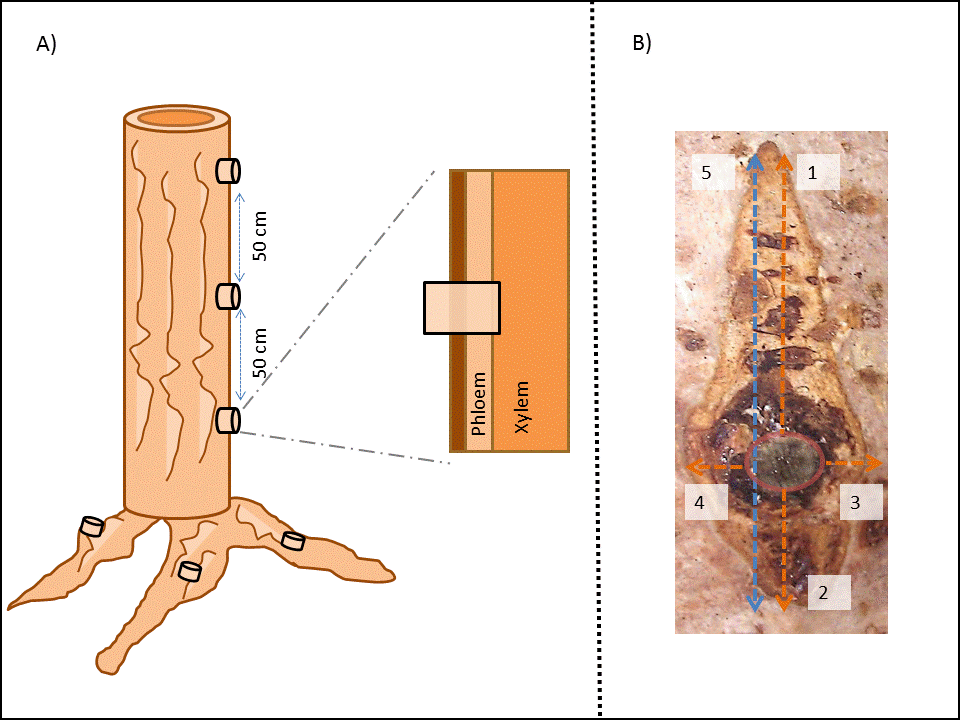
\includegraphics[bb=0cm 0mm 960bp 720bp,scale=0.4]{C:/Users/user/Documents/Courses/Thesis/schematicswip}

\emph{\footnotesize{}\protect\caption{{\footnotesize{}Schematic representation of inoculations (A) on stem
and roots, and measurements taken (B) from resulting lesions after
the experiment. In (B), measurements are for lesions extension upwards
from inoculation dowel (1), extension downwards from inoculation dowel
(2), extension to right or left from inoculation dowel (3,4), and
total length of the lesion (5) . The red circle in (B) outlines the
inoculation dowel. }}
}
\end{figure}



\subsection{Analysis of Data}

Preprocessing of the data was necessary to properly format the data,
and to ensure that the data was suitable for subsequent statistical
analysis. For the purposes of the analysis of the size of visible
lesions, i.e. the total length of the lesion and total width of the
lesion are used as the primary response variables. To create a single
response variable with which to characterize the lesions of the individual
tree, the lesions are conceptualized as 2-dimensional rectangles based
on the total length and maximal width of the lesion as measured from
the center of the inoculation point. 

Let $x_{1}$ be the total length of the lesion for a given measurement
and $x_{2}$ be the width. The geometric response, $y$ is described
by equation \ref{eq:1}.

\begin{equation}
y=(x_{1}x{}_{2})\label{eq:1}
\end{equation}


Analysis of the data  was conducted using R 3.1.2 (R Core Team, 2014),
and packages lme4 \citep{Bates2013}. Summary statistics and general
overview of the data is available in the results section. Welch's
two sample t-test was used to determine if differences existed between
the different directions of lesion growth. A linear mixed effects
model was used to determine the effects that the categorical variables
of site, tree, organ, and tissue had on tree response to the treatment.
As repeated measurements from a single subject (e.g., tree) cannot
be assumed to be independent of one another, explicit nesting was
specified in building the model to ensure accurate interpretation
of the model results. Linear mixed effects models allow for the broad
analysis of data which takes on complex, interrelated levels. 

The mixed effects model takes the form:

{\large{}
\begin{equation}
y=X\beta+Z\gamma+\epsilon\label{Eq 2: The Mixed Effect Model}
\end{equation}
}{\large \par}

where $y$ is the\emph{ }model estimate for the expected \textbf{Geometric}\textbf{\emph{
Response}},{\large{} $X$} is the design matrix of the observed fixed
effects variables (\textbf{\emph{Site, Treatment, Organ, Tissue)}},{\large{}
$\beta$} is the vector of the fixed effect coefficients, {\large{}$Z$}
is the design matrix of random effect variables (\textbf{\emph{Tree,
Organ }}\emph{within}\textbf{\emph{ Tree, Sample }}\emph{within}\textbf{\emph{
Organ }}\emph{within}\textbf{\emph{ Tree)}},{\large{} $\gamma$ }is
the vector of the random effects coefficients, and {\large{}$\epsilon$}
is a vector of residual errors. The responses are assumed to be drawn
from a normal distribution. 

Graphics were composed with R 3.1.2 and packages ggplot2, lattice,
and gridExtra \citep{Auguie2012,Hadley2009,Sarkar2008a}.. Exploratory
analysis with histograms and other charting techniques was utilized
to explore the structure and nature of the data along all steps of
modeling. A discussion of potential outliers as well as the effects
they have on the outcome of the model is given in the appendix; because
it was not possible to address the causes for several outliers present
in the data, the data was left intact for the primary analysis. To
check normality of the response variable, $y$, a Q-Q plot was created,
and when data visually violated assumptions of normality, a log natural
transform was used to attempt to bring the data into conformation
of the normal distribution, and a subsequent histogram was utilized
to verify the changes in the response variable. In elementary statistics
comparing the sizes of lesion measurements, a constant of 1.0 mm was
added to all measurements to correct in rare instances where no visible
lesion growth presented in one of the directions measured. \pagebreak{}


\section{Results}


\subsection{Summary Statistics for Lesions}



The mean lesion sizes are presented in Table 1. The mean lesions upwards
are generally consistent across sites. However, downwards lesions
are slightly larger for infected samples in Rovaniemi versus Lapinjärvi,
although the difference is not significant (\emph{t}=-0.40, \emph{D.F}.
=717.334, \emph{p}=0.68). Width is higher in Lapinjärvi infected trees,
but the difference is not significant (\emph{t=}-0.96, \emph{D.F}.
=693.57,\emph{ p=}0.33). There is no difference between the mean sizes
of the upwards or downwards lesion measurements (\emph{t=}1.31\emph{,
D.F}. =1432.67, \emph{p=0.18). }

\begin{table}[H]
\protect\caption{Mean Lesion Measurements $\pm$Standard Deviation}


\noindent %
\begin{tabular}{rrrrr}
\toprule 
\multicolumn{5}{c}{\textbf{Lesion Extension}}\tabularnewline
\midrule
\textbf{\footnotesize{}Site} & \textbf{\footnotesize{}Upwards (mm)} & \textbf{\footnotesize{}Downwards (mm)} & \textbf{\footnotesize{}Width (mm){*}} & \textbf{\footnotesize{}Total Length (mm){*}}\tabularnewline
\emph{\small{}Lapinjärvi} &  &  &  & \tabularnewline
\emph{\footnotesize{}Infected} & \textit{\footnotesize{}$19.3\pm15.0$} & \textit{\footnotesize{}$16.8\pm9.1$} & \textit{\footnotesize{}$16.0\pm5.0$} & {\footnotesize{}$45.5\pm21.8$}\tabularnewline
\emph{\footnotesize{}Control} & \textit{\footnotesize{}$5.9\pm6.6$} & \textit{\footnotesize{}$7.4\pm12.1$} & \textit{\footnotesize{}$12.0\pm4.0$} & {\footnotesize{}$22.2\pm17.1$}\tabularnewline
\emph{Rovaniemi} &  &  &  & \tabularnewline
\emph{\footnotesize{}Infected} & \textit{\footnotesize{}$19.0\pm14.7$} & \textit{\footnotesize{}$19.2\pm12.9$} & \textit{\footnotesize{}$12.0\pm5.0$} & {\footnotesize{}$48.1\pm25.9$}\tabularnewline
\emph{\footnotesize{}Control} & \textit{\footnotesize{}$5.4\pm4.1$} & \textit{\footnotesize{}$6.2\pm6.1$} & \textit{\footnotesize{}$12.0\pm3.0$} & {\footnotesize{}$20.4\pm8.6$}\tabularnewline
\bottomrule
\end{tabular}

\begin{singlespace}
\noindent \emph{\small{}{*}Measurement includes the inoculation dowel
width as well as lesion extension.}\end{singlespace}
\end{table}


Mean lesion size of the geometric response variable overall for site,
as well as for treatments within the site are presented in table 2.
Both field sites have highly similar lesion sizes in the geometric
response variable used for the mixed effects model in, as well as
similar lesions sizes across treatments by the different sites. 

\begin{table}[h]
\protect\caption{Mean Geometric Lesion Response, $y$}


\begin{tabular}{cc}
\toprule 
\multicolumn{2}{c}{\textbf{Lesion Geometric Response }}\tabularnewline
\midrule 
\textbf{Site} & \textbf{Mean $(mm^{2})$ $\pm SD$}\tabularnewline
\midrule
\emph{Lapinjärvi} & \textit{\footnotesize{}$6.0\pm0.8$}\tabularnewline
\emph{\footnotesize{}Infected} & \textit{\footnotesize{}$6.4\pm0.6$}\tabularnewline
\emph{\footnotesize{}Control} & \textit{\footnotesize{}$5.4\pm0.6$}\tabularnewline
\emph{Rovaniemi} & \textit{\footnotesize{}$6.0\pm0.7$}\tabularnewline
\emph{\footnotesize{}Infected} & \textit{\footnotesize{}$6.4\pm0.7$}\tabularnewline
\emph{\footnotesize{}Control} & \textit{\footnotesize{}$5.5\pm0.5$}\tabularnewline
\bottomrule
\end{tabular}
\end{table}


Figure 2 is a boxplot of the geometric response variable across sites
and treatments. Variability between trees which were infected appears
greater than control trees. Control trees appear to have lower general
variation in lesion sizes.

\begin{figure}[H]
\noindent \centering{}\includegraphics[clip,scale=0.75]{\string"C:/Users/user/Documents/Courses/Thesis/Figures for thesis/BoxplotGeomRespSeperate\string".pdf}\protect\caption{\emph{\small{}Boxplot of the geometric response as measured in both
sites. Points indicate observations outside the inter-quartile range.
The effect of treatment is significant (F=161.43, D.F. =1, Pr(>F)=
<0.00}{\small{}1)}}
\end{figure}


\pagebreak{}


\subsection{Linear Mixed Model for Lesion Geometric Response}


\subsubsection{Model Structure}

The response variable for the model is the $log_{e}$ transformed
product of the total length of the lesion and total width of the lesion
(see equation 1). Main (fixed) effects for the model structure are
the effect of treatment (control or infected), site (Rovaniemi or
Lapinjärvi), organ (stem or root), and tissue (phloem or xylem). Additionally,
all two way interactions between main effects were included. Random
effects included in the model were accounted for in three separate
grouping variables; tree level groupings, organ within tree level
groupings, and sample within organ within tree level groupings. 


\subsubsection{Fixed Effects}

Summary of the parameter estimates, confidence intervals for parameter
estimates (95\%), standard error of the samples parameter estimates,
and \emph{P}-values for the parameter estimates are given in Table
3. 

The intercept, i.e. the grand mean for all trees is the largest contribution
to lesion sizes, and is statistically significant (\emph{F}=23113.25,
\emph{P}=<0.001). Lesion sizes did not vary significantly between
the two field sites (\emph{F}=0.14, \emph{P}=0.71), nor did the size
of lesions vary between root and stem organs (\emph{F}=0.47, \emph{P}=0.49).
However, lesions did vary between xylem and phloem tissues (\emph{F}=353.35,
\emph{P}=<0.001), with xylem tissues having less total necrosis than
phloem tissues. No difference in lesion sizes occurred in the interaction
between treatment and site. However, the interaction between treatment
and organ varied significantly (\emph{F}=12.95, \emph{P}=<0.001),
with stems which were wounded (mock inoculated) expressing smaller
lesions sizes. The interaction between treatment and tissue did not
vary significantly (\emph{F}=0.61,\emph{ P}=0.47). The interaction
between site and organ varied marginally, with Rovaniemi stems expressing
larger lesion sizes (\emph{F}=5.99, \emph{P}=0.02). The response of
tissues between sites varied significantly (\emph{F}=33.52, \emph{P}=<0.0001),
with xylem tissues in Rovaniemi expressing larger lesions. Lastly,
the interaction between organs and tissues was significant \emph{(F}=6.96,
\emph{P}=0.009), indicating that stem xylem tissues expressed smaller
lesion sizes. . 

\begin{landscape}

\begin{table}[H]
\protect\caption{Parameter Estimates for Fixed Effects in the Lesion Response Model}


\begin{tabular}{lcccccc}
\hline 
\textbf{\emph{Fixed Effect}} & \textbf{\emph{Estimate}} & \textbf{\emph{Standard Error}} & \textbf{\emph{C.I 2.5\%{*}}} & \textbf{\emph{ C.I. 97.5\%{*}}} & \textbf{\emph{F}} & \textbf{\emph{P-value{*}{*}}}\tabularnewline
\hline 
\textit{\textcolor{black}{\emph{\small{}Intercept}}} & 6.659 & 0.096 & 6.476  & 6.842 & 23113.25 & <0.001\tabularnewline
\textit{\textcolor{black}{\emph{\small{}Treatment-Wounding}}} & -0.788 & 0.127 & -1.039  & -0.513 & 161.44 & <0.001\tabularnewline
\textit{\textcolor{black}{\emph{\small{}Site-Rovaniemi}}} & -0.270 & 0.127 & -0.508  & -0.020 & 0.14 & 0.71\tabularnewline
\textit{\textcolor{black}{\emph{\small{}Organ-Stem}}} & 0.084 & 0.106 & -0.129 & 0.293 & 0.47 & 0.49\tabularnewline
\textit{\textcolor{black}{\emph{\small{}Tissue-Xylem}}} & -0.455 & 0.043 & -0.534 &  -0.375 & 353.35 & <0.001\tabularnewline
\textit{\textcolor{black}{\emph{\small{}Treatment:Wounding{*}Site:Rovaniemi}}} & 0.055 & 0.156 & -0.247 &  0.345 & 0.12 & 0.72\tabularnewline
\textit{\textcolor{black}{\emph{\small{}Treatment:Wounding{*}Organ:Stem}}} & -0.432 & 0.120 & -0.656 & -0.187 & 12.95 & <0.001\tabularnewline
\textit{\textcolor{black}{\emph{\small{}Treatment:Wounding{*}Tissue:Xylem}}} & -0.033 & 0.043 & -0.120  & 0.053 & 0.61 & 0.47\tabularnewline
\textit{\textcolor{black}{\emph{\small{}Site:Rovaniemi{*}Organ:Stem}}} & 0.294 & 0.120 & 0.058  & 0.517 & 5.99 & 0.02\tabularnewline
\textit{\textcolor{black}{\emph{\small{}Site:Rovaniemi{*}Tissue:Xylem}}} & 0.249 & 0.043 & 0.164 & 0.328 & 33.52 & <0.0001\tabularnewline
\textit{\textcolor{black}{\emph{\small{}Organ:Stem{*}Tissue:Xylem}}} & -0.113 & 0.043 & -0.197 & -0.026 & 6.96 & 0.009\tabularnewline
\hline 
\end{tabular}

\emph{{*}C.I. = 95\% bootstrapped confidence intervals represented
at the 2.5\% and 97.5\% intervals. Calculated utilizing the ``confint''
function in lme4 package (Bates et. al.) with 1000 simulations}. 

\emph{{*}{*} P-value is the adjusted p-value calculated according
to the Kenword-Roger approximation to account for multiple comparisons}
\end{table}


\end{landscape}


\subsubsection{Random Effects}

The random effects of the groups and nesting are summarized in Table
4. The standard deviation for nested groups increases with levels
of the nesting going from individual trees, to samples nested in organs
nested in trees. Residual standard deviation is higher than the standard
deviation within trees, and higher than the standard deviation of
organ nested within tree. 

\begin{table}[H]
\protect\caption{Random Effects}


\begin{tabular}{cccc}
\toprule 
\textbf{\emph{Random Effects}} & \textbf{\emph{Type}} & \textbf{\emph{Variance}} & \textbf{\emph{Std. Deviation}}\tabularnewline
\midrule
Sample:(Organ:Tree) & Group Intercept & 0.149 & 0.386\tabularnewline
Organ:Tree & Group Intercept & 0.044 & 0.210\tabularnewline
Tree & Group Intercept & 0.037 & 0.194\tabularnewline
Residual & -- & 0.083 & 0.289\tabularnewline
\bottomrule
\end{tabular}
\end{table}


Plots of the group specific random effects are shown in Figure 3.
The plot allows the visualization of the random effects from the model
in all the grouping levels. Group labels are not present for the first
two grouping dotplots, as there are 360 and 120 distinct group random
effects estimated for these, respectively. The highest level of grouping
(Tree) has individual labels represented on the y-axis, and the most
and least susceptible trees as modeled are easily determined. The
variance increases with the levels of grouping; samples within organ
have the highest variances, and tree level variance is the lowest
of the random effects.

\begin{figure}[H]
\includegraphics[width=1\columnwidth,height=0.4\paperheight]{\string"C:/Users/user/Documents/Courses/Thesis/Figures for thesis/ranefplots\string".pdf}

\protect\caption{\emph{Ordered Dotplots of the Model Random Effects}}
\end{figure}



\subsection{Model Validation and Diagnostics}

\begin{figure}
\includegraphics[scale=0.65]{\string"C:/Users/user/Documents/Courses/Thesis/Figures for thesis/DensityPlotParametersPDFBW\string".pdf}

\protect\caption{Profiled Likelihood of Parameter Estimates }
\end{figure}


The likelihood of the parameter estimates are presented in Figure
4. Profiles were created utilizing the ``profile'' function in lme4
package. Reviewing the ranges and densities of the profile plots gives
an indication of the likelihood of the parameter estimate being equal
to a value given the observed data, as well as the variability in
the likelihood of observing differing values of the parameter estimates.
Parameter profiles were normally distributed, with some kurtosis evident
in the random effects standard deviation estimates for residual variance,
tree, organ within tree, and sample within organ within tree groupings
($\sigma,\sigma_{1},\sigma_{2},\sigma_{3,}$ in Figure 4, respectively).
Other profiles of parameter likelihood (e.g. those representing fixed
effects) show little to no kurtosis. Ranges of the profiled parameters
strongly coincide with the 95\% confidence intervals presented in
Table 3, and maximal likelihoods in the generated profiles are at
the original parameter estimates. 

Model goodness of fit was examined by plotting the observed values
for the geometric response against the fitted values from the model
(Figure 5). Marginal $R^{2}$ is 0.496, or 49.6\% of total variance.
Conditional $R^{2}$ is 0.866, or 86.6\% of total variance. The inclusion
of the random effects in the model accounts for 0.370, or 37.0\% of
variance in the data %
\footnote{The $R^{2}$ measure commonly utilized for linear regressions is not
directly applicable to mixed effects models. However, \citet{Nakagawa2013}
suggested a new method of calculating $R^{2}$ for mixed effects models
which separates the influences of the fixed effects and random effects
into two measures; marginal $R_{lmm(m)}^{2}$ and conditional $R_{lmm(c)}^{2}$.
Marginal $R_{lmm(m)}^{2}$ represents the variance attributed to the
fixed effects only. Conditional $R_{lmm(c)}^{2}$. includes both the
influence from the fixed effects as well as the random effects in
the given model. %
}. 

Overall model fit was subjectively good, with 86.6\% of total variance
explained. The total proportion of variance explained by the fixed
effects accounts for a greater proportion of the total variance explained
by the model than does the random effects (49.6\% versus 37\%). However,
random effects for the model still account for a large portion of
the variance explained in the model, indicating that their inclusion
is informative in the context of modeling lesion responses in \emph{P.
abies}.

\begin{figure}[H]
\noindent \centering{}\includegraphics[clip,scale=0.5]{\string"C:/Users/user/Documents/Courses/Thesis/Figures for thesis/ModelFitPlot\string".pdf}\protect\caption{\emph{Plot of the estimated ($\hat{y}$) versus observed ($log_{e}(y)$)
values of the geometric response variable from the mixed effects model}}
\end{figure}


\pagebreak{}


\section{Discussion}

Based on the results, this study concludes that differences in lesion
sizes are not likely to be due to differences between the sites. However,
readers would do well to note that many aspects of this study are
subject to analysis only in the context of the collected data and
experiment performed herein, and thus broad based inferences upon
the effects of historical isolation from pathogen as a potential factor
for differences in lesion response in \emph{P. abies} to \emph{H.
parviporum} should not be drawn from this study alone. These results
partially coincide with work carried out by \citet{Witzell2011},
which loosely concluded that difference in geographic origin might
not affect overall resistance of \emph{P. abies }to \emph{H. annosum
s.l.} However, their study explored the ability of \emph{H. annosum
s.s.} versus \emph{H. parviporum }to colonize in different geographical
locations with differing temperature regimes, but did not look at
regions where the fungus was not known to be present prior to the
study. 

This study found no evidence for the effect of organ on the response
in lesion size. However, other studies, including \citet{Kerio2015}\emph{,}
have concluded that a difference exists in the response of \emph{P.
abies }between roots and stems. Reasons for a lack of similar findings
in this study could be attributed to many possible factors, such as
soil type, temperature and climate, time between inoculation to harvest,
and relative ability of the fungal strain to overcome host responses.
However, as the natural pathway for infection of \emph{H. annosum
s.l.} is through the roots, it is somewhat surprising that a difference
is not present in this study. One possible explanation for this observation
is due to the sizes of roots inoculated. In Rovaniemi, the sizes of
roots utilized for the inoculations was significantly smaller than
the average root sizes in Lapinjärvi; a study by Garbelotto and Slaughter
(1997), found a positive correlation between root diameter and fungal
growth. Refitting the model using only data from the Lapinjärvi or
Rovaniemi field sites does change the significance of the organ variable;
in Lapinjärvi the variable is a significant predictor, whereas in
Rovaniemi it is not, indicating that perhaps the smaller sizes of
roots in Rovaniemi are the reason for a lack of significance of the
organ variable in the model utilizing both field sites. . 

It is worth noting that most studies where artificial inoculations
have been performed on \emph{P. abies }with \emph{H. annosum s.l.
}focused solely on stem inoculations, which does not mimic the natural
infection pathway in \emph{H. annosum s.l.} Because of this, it can
be difficult to judge whether or not a difference is generally assumed
to exist in the responses between the two organs based on the results
of the few studies which have explored root inoculations. Further
complications occur due to the highly variable root structure and
variability in root sizes utilized for inoculation points in this
study, as well as the lack of control for genotype in this study. 

The difference in lesion response in tissues was significant in this
study. In the study conducted by \citet{Kerio2015}\emph{, }no difference
was noted between tissues. However, different anatomical features
are present in the different tissues, which may influence the ability
of \emph{H. annosum s.l. }to grow in the separate tissues \citep{Krekling2004}.
 Further reasons for the observed difference in the response between
differing tissues could be due to a number of different factors; genetic
control of the sample subjects in future experiments could help to
determine if the observed differences are due to genetic, environmental,
or latent factors. 

Several of the statistical interactions in this study were found to
be significant influences upon the response of \emph{P. abies }to
infection with \emph{H. parviporum. }The interaction between treatment
and organ was significant, with stems being less susceptible to wounding
than roots. This is in contrast to other studies which have examined
the response of organs to inoculation, which have found significant
differences in the treatment by organ, e.g. \citet{Kerio2015}, which
found stem lesions more susceptible to wounding than root lesions.
Furthermore, the interaction between site and organ was found to be
marginally significant, with stems lesions in Rovaniemi being larger.
This could be due to a number of factors which were unaccounted for
in this study. Norway spruce has high genetic plasticity, which could
potentially account for differences in the response of the organs
at various sites \citep{Chen2012,Reich1996}. However, the design
of the study did not control for genotype of phenotype diversity,
so there is no way to account for this variance in the study as it
was executed. Other possible reasons why a different response by organ
was different by site could be due to differences in the overall size
of the trees, as trees of differing sizes and ages may respond differently
to infections.


\subsection{Experimental Design Limitations}

The biggest limitation in the study is the lack of clonal material.
Although the results of the study may be sufficient for drawing broad-based
conclusions about aspects of the defense response of Norway spruce
to infections with \emph{H. parviporum} in natural settings, it is
not possible to conclude what aspects of an individual in the study
contributed to more or less susceptibility. Clonal material would
have allowed a better assessment of the influence and variability
of individual tree's phenotypes. For example, if a tree on whole shows
a strong resistance or susceptibility to the infections, with non-clonal
material it is not possible to infer if this is the result of the
trees phenotype, or whether it would be expected to see this variation
naturally in a sufficiently large sample of clonal material. This
lack of clonal material is a principal reason why trees in this study
are treated as random effects as opposed to fixed effects; in a study
controlled for tree genotype with sufficient numbers of ramets per
clones, it would be possible to draw stronger conclusions about the
resistance of individual Norway spruce genotypes to \emph{H. parviporum}.

The lack of control over genetics makes it difficult to know what
to do with outliers present in the data; for this reason, several
outliers in the traditional sense were kept in the analysis. Trees
RT2 and LT8 showed extreme resistance and susceptibility to treatment,
respectively. Tree LW8 had decay due to a natural fungal infection\emph{
}prior to the experiment, but it was only noted when the tree was
cut down for processing. If clonal material was utilized, it would
be possible to determine if the tree genotype was really susceptible,
or if this was an unnatural response to the treatment. Tree RT2 was
abnormally resistant to infection, but again it is not possible to
deduce the reasons as to why. Because it is not possible to deduce
the causes for responses of trees such as RT2 and LW8, which display
extreme responses with this studies experimental design, it may not
be appropriate to remove the suspected outliers from the analysis;
for this reason, these trees and all samples from them were kept in
the analysis. 

The potential effects of historical isolation from the pathogen based
on latitude could not accurately be determined based on this study's
experimental design. Too many confounding factors could account for
any potential observed differences, even though this study found no
difference between tree responses between sites. Additionally, only
one site in each geographical region was utilized for the study; to
effectively determine the effects of a site factor, more than one
replicate for each area (i.e. areas where \emph{H. annosum s.l. }are
known to naturally infect trees, versus one where \emph{H. annosum
s.l. }are not known to be present) is necessary. However, a previous
study by \citet{Karlsson2008} indicated that differences in resistance
do exist between geographic areas; two sites in southern Europe utilizing
clonal material (Greece and Italy) had significant correlations between
fungal growth, lesion size and other indicators of resistance, while
a third field site in Sweden utilizing the same clonal material did
not share significant correlations with the southern European field
sites. However, the authors speculated that environmental factors
could be responsible for the lack of correlations between the two
regions. Further studies could attempt to address differences between
trees acclimatized to certain growing environments by using a crossed
design wherein trees from both genetic origins are utilized across
field sites.

Further issues with the experimental design for this study include
a lack of control of external factors such as different flora and
fauna at the sites could have implications in the estimation of site
based effects. This is one major complication with carrying out field
based experiments as opposed to those which take place in highly controlled
laboratory and greenhouse settings. Temperature, weather events, and
other natural influences are not generally controllable in field experiments.
However, for drawing ecological conclusions regarding the interactions
between Norway spruce and \emph{H. annosum s.l., }it is useful to
carry out field experiments; any resulting residual variances can
then be attributed to uncontrollable environmental factors, but would
require that the experimental design properly controlled for both
the host genotype and site factor. 


\subsection{Potential Issues in the Analysis}

Data analysis, in many instances, becomes a subjective task as opposed
to a purely objective one; parsimony is something to strive for in
any analysis. In this study, the choices taken in regards to the methodology
utilized for analyzing and presenting data were based on balancing
several conflicting goals: how to best characterize the lesion response
on various levels, while avoiding over parametrization of the model,
and maintaining interpretability. 

In this study, the response of interest is the lesion size as in indication
of resistance or susceptibility for a given sample, with inferences
then drawn for the different tissues, organs, and individual tree.
In reality, the lesion presents as a three dimensional reaction to
the inoculation. However, to analyze the lesions, a simplified view
of the lesions was utilized, conceptualizing the lesions as a rectangular
area based on maximal width and length measurements across the point
of inoculation. Lesions from the inoculations presented in many ways,
and no single geometric shape is consistent across lesions. In hindsight,
there are better, albeit much more time consuming ways, to measure
the lesions. With proper photographic equipment and software, it would
be possible to measure accurately the entire area of the lesion without
needing to resort to constricting the conceptualization of the lesion
to a single shape, utilizing a known measurement (i.e., measuring
the samples on a white background with a ruler / scale) as a calibration.
Implementing this could increase the accuracy of the parameter estimates,
as well as better characterize the actual lesions by calculating a
highly accurate area measurement. This technique has been applied
in other studies with agricultural plants, but to the best of the
author's knowledge, has not been implemented in studies examining
lesions created from \emph{H. annosum s.l.}

Outliers are of special concern, as their presence in data can modify
parameter estimates. In this study, outliers were still included in
the analysis. Nevertheless, to ignore the possibility of the influence
of several observations which traditionally might be considered outliers
would be remiss. The potential influence of outliers is examined in
the appendix. 


\subsection{Uncertainty in Results}

Methodologies for performing and assessing the effects of \emph{H.
annosum s.l}. on conifers vary, and thus conclusions and results between
studies can be difficult to generalize. Differences in experimental
design include ways in which the inoculation is performed. Deep tissue
wounding has been used in various studies, and is done by boring directly
to the heartwood of a living tree to introduce to the pathogen directly
to susceptible tissues, which was the technique utilized for this
study \citep{Delatour1998}. In a separate inoculation technique,
superficial wounding targets only the surface of the cambium of the
tree which is inoculated with the pathogen \citep{Delatour1998}.
Other variables in studies examining the resistance in conifers to
\emph{H. annosum s.l. }include number of replicates per tree, location
of field sites, temperature profiles of the regions where experiments
are performed, choices of clonal material, length of incubation times,
and methods for analyzing the resulting data. However, research indicates
that overall sizes of respective lesions in inoculated clones may
be a good proxy for indicating resistance or susceptibility to infections
from \emph{H. annosum s.l.} \citep{Woodward2007,Swedjmark1997,Delatour1998}\emph{.}

Although the analysis is relatively appropriate for the data collected
in this study, and does an acceptable job characterizing the lesions
as well as the variance present in the study which are under controllable
factors (i.e., treatment, organ, and tissue), the mixed effects approach
does little to interpret the potential resistance or susceptibility
of the trees on a biological level beyond looking at overall lesion
sizes. Furthermore, the lack of control for tree genotype is a troubling
shortcoming in this study which prevents anything beyond generalization
about tree resistance to be drawn from this data. In future studies,
use of clonal material would be essential for comparing the resistance
across treatments. Furthermore, molecular methods could be utilized
to explore in depth measures of resistance. For example, analysis
of RNA transcripts to determine up-regulated gene products such as
chitinase, terpenes, and other PR-family proteins, etc., in resistant
versus susceptible trees. The use of molecular methods in conjunction
with analysis of lesions would provide more detailed information about
not only the resistance of trees characterized as a molecular response,
but would also allow for correlations to be made between specific
gene products and lesion characteristics. Previous studies have incorporated
analysis of lesions and fungal growth within host tissues, along with
molecular methods for assessing various aspects of tree resistance
to \emph{H. annosum s.l.} \citep{Woodward2007,Hietala2003}. This
study did not analyze the actual growth of the fungus in relation
to the size of the lesion response, which could be done in further
work as an additional way to characterize the resistance levels of
individual trees to infection.

In hindsight, it is difficult to consider latitude as a reasonable
effect to study for the resistance of Norway spruce to \emph{H. parviporum};
in reality, isolation from historical presence of the pathogen is
the parameter this study attempted to address, and subsequent studies
should look at this along with specific environmental factors which
may influence the pathology during the experiment.


\section{Conclusions}

\emph{H. annosum s.l.} is a devastating forest pathogen which causes
millions of euros in losses to timber products annually. Many factors
contribute to the capability of the pathogen to proliferate and spread
under natural conditions, and, despite research into forest tree breeding
for resistance and use of various control methods, the pathogen still
causes huge damages economically, and continues to be a leading concern
in the modern forestry sector. Understanding the different aspects
of the epidemiology and life cycles of both the host and pathogen
may hold key information to combating infections and breeding for
improvements in resistance. Factors such as genetic origin, tree age
and size, as well as environmental conditions all impact the resistance
of Norway spruce to infection to \emph{H. annosum s.l.}

The study described in this thesis attempted to address several aspects
of the resistance potential of \emph{P. abies }to \emph{H. parviporum
}in natural conditions. Primary factors examined as the research for
this project were the effects of site across areas where the pathogen
is both known to be present as well as an area where the pathogen
does not have a known historical presence. Additional factors examined
in this research include the potential for difference responses in
both host tree organ (root and stem), tissues (phloem and xylem),
as well as the statistical interactions between various crossed factors
included in the design of the experiment. 

The study found that overall, Norway spruce resistance does not appear
to differ between the two field sites, and in this regard, the study
concludes that resistance does not appear to vary in Norway spruce
populations which are not known to have high rates of natural infection
versus area in which the pathogen has a recent historical presence.
Future studies should incorporate stricter controls, i.e., the use
of clonal materials, and if possible, crossing of geographic origin
of the clonal material across environmentally distinct field sites
in attempt to better address the influence of geographic isolation
from the pathogen in recent history. Further research into site based
differences should also account for different environmental and soil
based conditions. 

The study did not find differences with regards to resistance based
on the whether the inoculation was performed in the stem versus the
root organ of a given tree. This is in contrast to other studies reviewed,
which did find a difference between root and stems in their susceptibility.
Future studies conducted in a similar matter should incorporate root
size measurements as a potential influential variable.

Findings of a difference in variability of resistance between tissues
in this study are in contrast with other studies examining the subject.
Exact reasons are uncertain, but possible explanations include genetics,
and environmental factors, among others. 

Finally, the use of a mixed effects model to analyze the complex nature
of the data collected proved to be a useful tool to interpret the
results, as well as to shed light onto the influences of accounting
for random effects in the modeling. Few other studies reviewed have
taken this approach to modeling lesion response of forest trees; further
studies may attain valuable additional information by including random
effects into their analysis and moving away from typical multiple
regression / ANOVA based analysis which collected data may violate
statistical assumptions for in these sorts of experiments. 

. 

\pagebreak{}

\begin{singlespace}
\noindent \renewcommand{\BIBand}{\&} \bibliographystyle{C:/Users/user/Documents/Courses/Thesis/bibgen}
\bibliography{C:/Users/user/Documents/library}

\end{singlespace}

\pagebreak{}

\appendix

\section*{Appendix 1\addcontentsline{toc}{section}{Appendix 1}\thispagestyle{empty}}

\setcounter{figure}{0} \renewcommand{\thefigure}{A.\arabic{figure}} 


\subsection*{Maps}

\begin{figure}[H]
\includegraphics[scale=0.7]{\string"C:/Users/user/Documents/Courses/Thesis/Figures for thesis/TopoLapinjarvi\string".png}\protect\caption{Map of Lapinjärvi Field Site}
\end{figure}


\begin{figure}[H]
\includegraphics[scale=0.7]{\string"C:/Users/user/Documents/Courses/Thesis/Figures for thesis/TopoRovaniemi\string".png}\protect\caption{Map of Rovaniemi Field Site}
\end{figure}
\index{Map of Lapinjärvi Field Site Map of Rovaniemi Field Site}

\pagebreak{}


\section*{Appendix 2 \addcontentsline{toc}{section}{Appendix 2}\thispagestyle{empty}}


\subsection*{Normality of Data and Outliers}

The geometric response variable violated assumptions of normality.
A natural logarithm transform was applied to the data resulting in
a much closer to normal structure of the data.

\begin{figure}[h]
\includegraphics[scale=0.7]{\string"C:/Users/user/Documents/Courses/Thesis/Figures for thesis/GeometricResponseHistograms\string".pdf}

\protect\caption{\emph{Histogram of the geometric response variable, $y$, and transformed
geometric response variable $log_{e}(y)$, indicating a lack of normality
in the uncorrected data.}}
\end{figure}


To determine if any trees had significant influence on the parameter
estimates, post hoc investigation of the random effect of tree level
groupings was performed. Cook's distance is a measure which is utilized
to examine the influence of a unit on all parameters. Using the value
of $4/n$, where n is the number of groups (in this case, trees) gives
a cutoff value of $0.066$ for determining overly influential observations.
Only tree RT2 is overly influential (see Figure A.4) when considering
the influence upon all fixed effects. 


\section*{Appendix 2}

\begin{figure}[H]
\includegraphics[scale=0.65]{\string"C:/Users/user/Documents/Courses/Thesis/Figures for thesis/CooksDist_Tree\string".pdf}\protect\caption{Cook's Distance for all Trees }
\end{figure}


\thispagestyle{empty}\pagebreak{}


\section*{Appendix 3\addcontentsline{toc}{section}{Appendix 3}\thispagestyle{empty}}


\subsection*{Model Comparison}

Several models were constructed before settling upon a final model.
To compare models, an ANOVA was used to select evaluate the most informative
model. However, as the calculation of degrees of freedom with restricted
estimate of maximum likelihood for random effects is non-trivial,
so models were refit using maximum likelihood. Three models were compared;
the most elementary model included only tree level random effects
groupings, and is specified in equation (3). The next model included
full specification of random effects as in the full model, but did
not include any interaction terms between fixed effects (4). The final
model contained full specifications of the random effects as well
as all two way interactions between fixed effects (5). The full model
including interactions as well as full specification of random effects
is significantly better than the other models ($\chi^{2}$= 271.13,
\emph{P = < 0.001).}

\noindent {\footnotesize{}
\begin{equation}
\hat{y}=Site+Treatment+Organ+Sample+random(Tree)\label{eq:Minimal Model}
\end{equation}
\begin{equation}
\hat{y}=Site+Treatment+Organ+Tissue+random(Tree/Organ/Sample)\label{eq:No Interactions}
\end{equation}
\begin{multline}
\hat{y}=Site*Treatment+Site*Organ+Site*Tissue+Treatment*Organ+\\
Treatment*Tissue+Organ*Tissue+random(Tree/Organ/Sample)\label{eq:Full Model}
\end{multline}
}{\footnotesize \par}

\begin{figure}[H]
\protect\caption{Model Comparisons Table}


\begin{tabular}{ll}
\hline 
Model Description & Pr > $\chi^{2}$\tabularnewline
\hline 
{\small{}(3) No Interactions, single random effect (Tree)} & {\small{}--}\tabularnewline
{\small{}(4) No Interactions, full random effects} & {\small{}1}\tabularnewline
{\small{}(5) Full model utilized in the study} & {\small{}< 0.001}\tabularnewline
\hline 
\end{tabular}
\end{figure}

\end{document}
